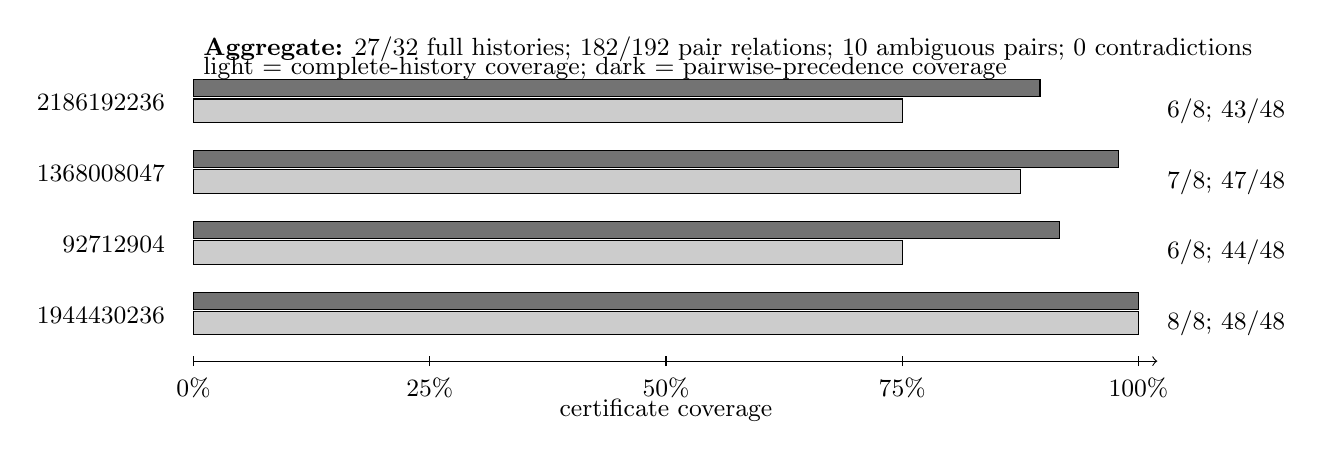
\begin{tikzpicture}[x=0.12cm,y=0.9cm, font=\small]
\def\xhist{84}
\def\xpairs{100}

\node[anchor=east] at (0,4) {2186192236};
\node[anchor=east] at (0,3) {1368008047};
\node[anchor=east] at (0,2) {92712904};
\node[anchor=east] at (0,1) {1944430236};

% full-history coverage bars, normalized to 100
\filldraw[fill=black!20] (2,3.72) rectangle (77,4.05); % 6/8 = 75
\filldraw[fill=black!20] (2,2.72) rectangle (89.5,3.05); % 7/8 = 87.5
\filldraw[fill=black!20] (2,1.72) rectangle (77,2.05);
\filldraw[fill=black!20] (2,0.72) rectangle (102,1.05); % 8/8

% pair coverage bars beneath each history bar
\filldraw[fill=black!55] (2,4.08) rectangle (91.58,4.32); % 43/48
\filldraw[fill=black!55] (2,3.08) rectangle (99.92,3.32); % 47/48
\filldraw[fill=black!55] (2,2.08) rectangle (93.67,2.32); % 44/48
\filldraw[fill=black!55] (2,1.08) rectangle (102,1.32); % 48/48

\node[anchor=west] at (104,3.88) {6/8; 43/48};
\node[anchor=west] at (104,2.88) {7/8; 47/48};
\node[anchor=west] at (104,1.88) {6/8; 44/48};
\node[anchor=west] at (104,0.88) {8/8; 48/48};

\draw[->] (2,0.35) -- (104,0.35);
\foreach \x/\lab in {2/0,27/25,52/50,77/75,102/100}{
  \draw (\x,0.28) -- (\x,0.42);
  \node[anchor=north] at (\x,0.25) {\lab\%};
}
\node[anchor=north] at (52,-0.05) {certificate coverage};

\node[anchor=west] at (2,4.75) {\textbf{Aggregate:} 27/32 full histories; 182/192 pair relations; 10 ambiguous pairs; 0 contradictions};
\node[anchor=west] at (2,4.48) {light = complete-history coverage; dark = pairwise-precedence coverage};
\end{tikzpicture}
